\chapter{\Peano's architecture}
\label{chapter:architecture}


\begin{center}
  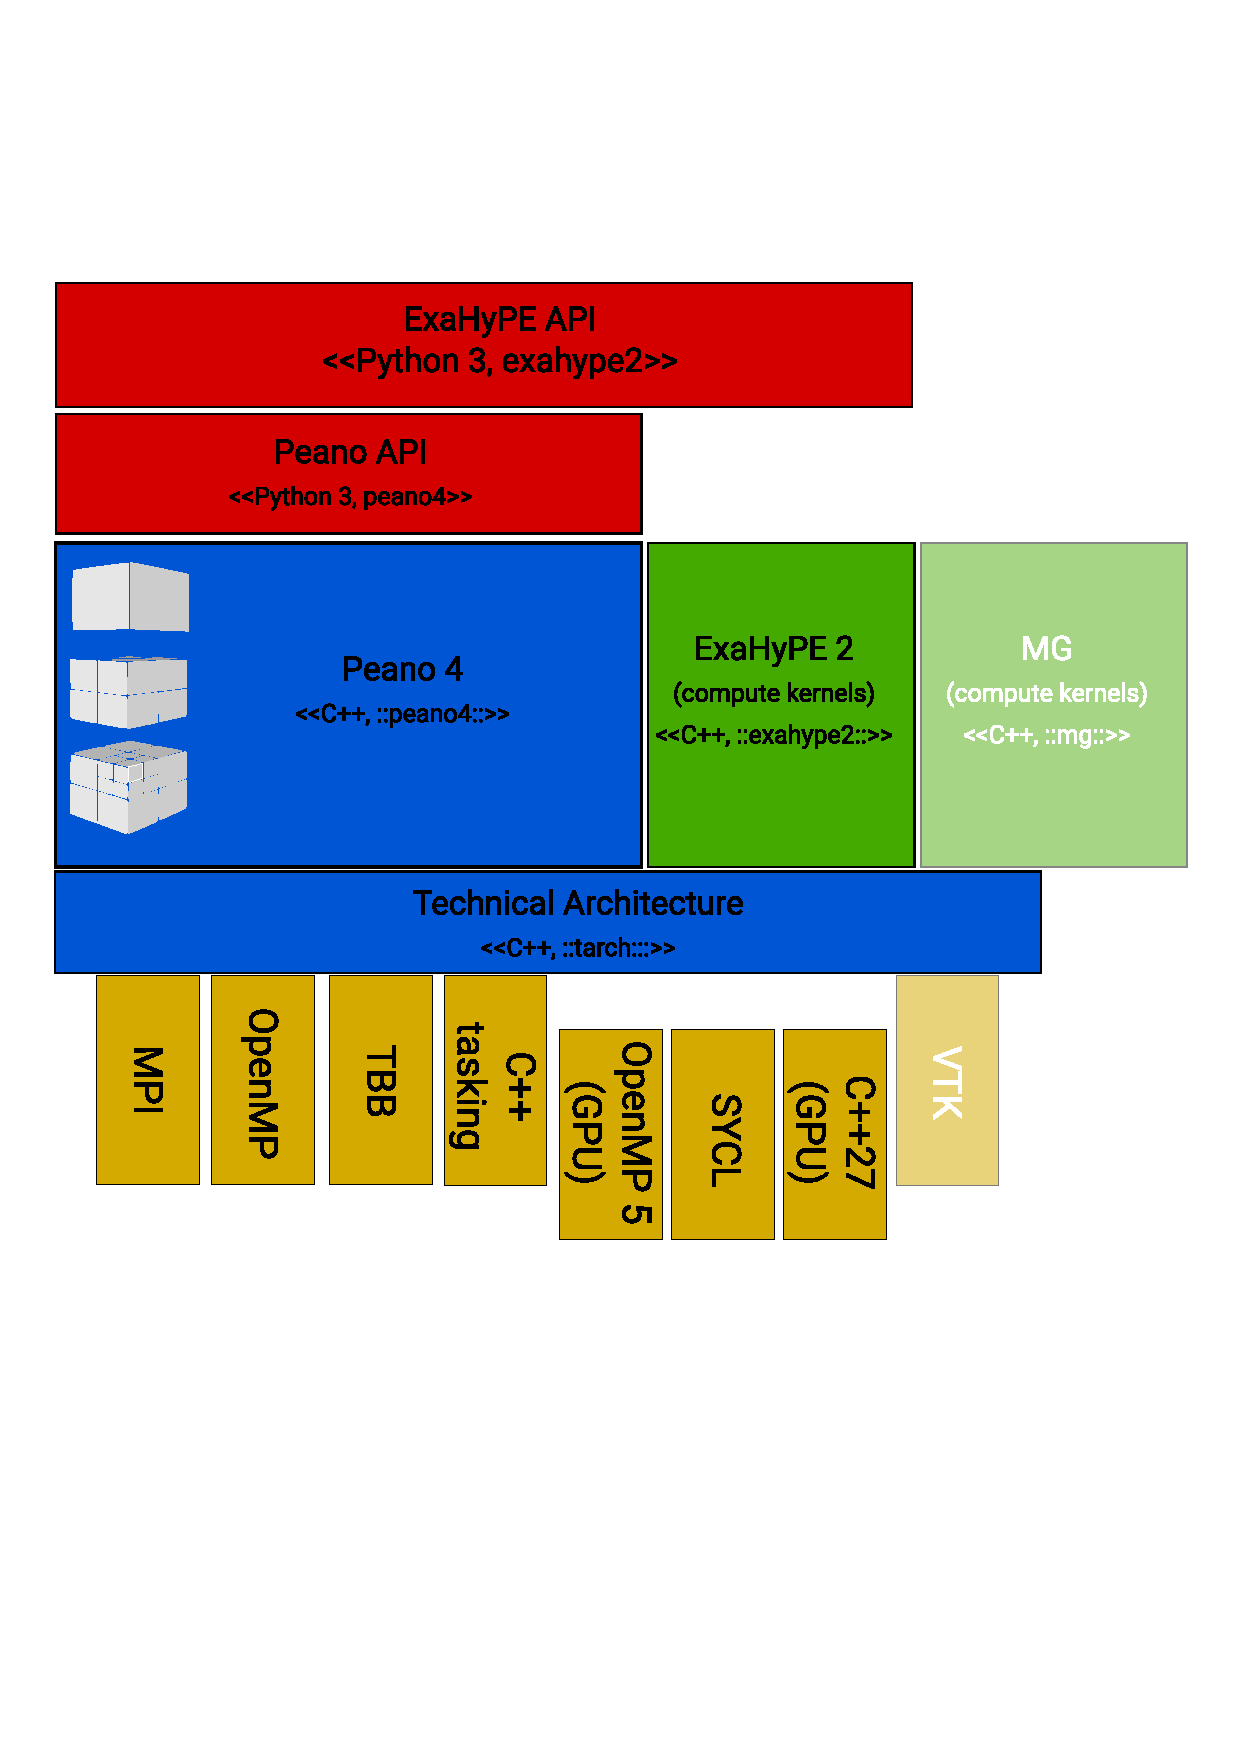
\includegraphics[width=0.6\textwidth]{../src/peano4/architecture-layers.pdf}
\end{center}


\noindent
\Peano\ is organised into layers, and only the bottom two layers are found in
all \Peano\ applications.
I discuss the layers bottom-up:

\begin{itemize}
  \item[tarch] The technical architecture is a set of loosly coupled building
  blocks that hide away technical details. There's for example a namespace to
  handle multicore parallelism, a logging component, or a collection of
  primitive linear algebra routines for small problems. It is written solely in
  C++ and its purpose is to hide away third-party dependencies such as OpenMP
  or MPI. I originally designed it as a stand-alone thing which is not tied to
  Peano though I'm not aware of any other project that currently uses it. The
  layer is pronounced ``T Arch'' and is encapsulated in a namespace
  \texttt{tarch}, as I didn't want to write the full name ``technical
  architecture'' every time.
  \item[peano4] The namespace \texttt{peano4} hosts the \Peano\ core. It is
  entirely written in C++ (using the tarch) and holds the heart and brain of the
  code, i.e.~all the data management, the tree traversals and the domain
  decomposition.
  \item[Native] \Peano\ applications use solely the core and the tarch. I write
  such codes from time to time myself, but it is a tedious task as all the user
  data management and management of ``which routine is used when'' has to be
  programmed manually.
  \item[Other projects] can obviously supplement the core and tarch with further
  routines using either of the two components. The most prominent project
  extending the core is maybe \ExaHyPE. The illustration here is not 100\%
  correct as noone forces developers to write these extensions in C++. In
  practice however, most of them are (with small Fortran imports, e.g.). 
  \item[Native projects] can use the core extensions using C++. Most projects
  (like ExaHyPE) however do all offer a more abstract interface (see below).
  \item[Python API] \Peano\ offers a Python API which is basically a code
  generator yielding lots of C++ snippets that plug into the core and use the
  tarch. Some of my examples use this Python API only.
  \item[API extensions] are also offered by other projects such as ExaHyPE or
  ExaClaw. They often supplement the core Python API with further classes.
\end{itemize}


\section*{Code organisation}

\Peano's core is a collection of static libraries. 
A \Peano\ application consists of C++ glue code which combines all of these
libraries.
This glue code is generated through the Python API.


\begin{itemize}
  \item[documentation] Hosts the \LaTeX\ sources of the document that you hold
  in your hands.
  \item[python] Holds the Python API scripts. Within the \texttt{python}
  subdirectory, you find scripts for both the \Peano\ core API, toolboxes and
  large-scale \Peano\ applications.
  \item[src] Holds the C++ Peano sources of the Peano core and all the
  toolboxes.
  \item[examples] Collection of simple examples. Most of them are hard-coded,
  stand-alone codes.
  \item[benchmarks] Collection of benchmark scripts.
  \item[applications] Proper, real-world applications.
\end{itemize}


